\documentclass[submit]{../harvardml}
\usepackage{../common}
 
\course{CS1810-S25}
\assignment{Homework \#5}
\duedate{April 18, 2025 at 11:59 PM}

\newcommand{\attr}[1]{\textsf{#1}}
\usepackage[OT1]{fontenc}
\usepackage[colorlinks,citecolor=blue,urlcolor=blue]{hyperref}
\usepackage{graphicx}
\usepackage{subcaption}
\usepackage{framed}
\usepackage{fullpage}
\usepackage{amsmath}
\usepackage{amssymb}
\usepackage{color}
\usepackage{todonotes}
\usepackage{listings}
\usepackage{bm}
\usepackage{tikz}
\usepackage{float}
\usepackage{pythonhighlight}
\usepackage[mmddyyyy,hhmmss]{datetime}
\usetikzlibrary{positioning,shapes,arrows}

\usepackage{float}

\lstset{
  language=Python,
  basicstyle=\small\ttfamily,
  frame=single,
  backgroundcolor=\color{white},
  breaklines=true,
  showstringspaces=false
}

\definecolor{verbgray}{gray}{0.9}

\lstnewenvironment{csv}{
  \lstset{backgroundcolor=\color{verbgray},
  frame=single,
  framerule=0pt,
  basicstyle=\ttfamily,
  columns=fullflexible}}{}

%%%%%%%%%%%%%%%%%%%%%%%%%%%%%%%%%%%%%%%%%%%
%% Solution environment
\usepackage{xcolor}
\newenvironment{solution}{
    \vspace{2mm}
    \color{blue}\noindent\textbf{Solution}:
}{}
%%%%%%%%%%%%%%%%%%%%%%%%%%%%%%%%%%%%%%%%%%%


\begin{document}

\begin{center}
{\Large Mixtures, EM, and Graphical Models}\\
\end{center}



\subsection*{Introduction}

This homework assignment will have you work with EM for mixtures, PCA, and graphical models.

\subsection*{Resources and Submission Instructions}

We encourage you to read sections 9.4 and 8.2.5 of the course textbook.

Please type your solutions after the corresponding problems using this \LaTeX\ template, and start each problem on a new page.

Please submit the writeup PDF to the Gradescope assignment `HW5'. Remember to assign pages for each question.  \textbf{You must include any plots in your writeup PDF. }. Please submit your \LaTeX file and code files to the Gradescope assignment `HW5 - Supplemental.' The supplemental files will only be checked in special cases, e.g. honor code issues, etc. Your files should be named in the same way as we provide them in the repository, e.g. \texttt{hw5.pdf}, etc.



\begin{problem}[Expectation-Maximization for Gamma Mixture Models: Derivations, 10pts]
  In this problem we will explore expectation-maximization for a Categorical-Gamma Mixture model. \\

  \noindent Let us suppose the following generative story for an observation $x$: first one of $K$ classes is randomly selected, and then the features $x$ are sampled according to this class. If $$z \sim \operatorname{Categorical}(\btheta)$$ indicates the selected class, then $x$ is sampled according to the class or ``component'' distribution corresponding to $z$. (Here, $\btheta$ is the mixing proportion over the $K$ components: $\sum_k \theta_k = 1$ and $ \theta_k > 0$.) In this problem, we assume these component distributions are gamma distributions with shared shape parameter but different rate parameters: 
  $$ x | z \sim \operatorname{Gamma}(\alpha, \beta_k). $$
  In an unsupervised setting, we are only given a set of observables as our training dataset: $\mathcal D = \{x^{(n)}\}_{n=1}^N$. The EM algorithm allows us to learn the underlying generative process (the parameters $\btheta$ and $\{\beta_k\}$) despite not having the latent variables $\{z^{(n)}\}$ corresponding to our training data.

  \vspace{1em}

  \begin{enumerate}
    \item \textbf{Intractability of the Data Likelihood.} We are
    generally interested in finding a set of parameters $\beta_k$ that
    maximizes the likelihood of the observed data: $$\log
    p(\{x^{(n)}\}^N_{n=1}; \btheta, \{\beta_k\}^K_{k = 1}).$$ Expand the data
    likelihood to include the necessary sums over observations
    $x^{(n)}$ and to marginalize out the latents
    $\boldz^{(n)}$. Why is optimizing this likelihood directly
    intractable?

    \item \textbf{Complete Data Log Likelihood.} The complete dataset
    $\mathcal D = \{(x^{(n)}, \boldz^{(n)})\}_{n=1}^N$ includes latents $\boldz^{(n)}$. Write
    out the negative complete data log likelihood: $$\mcL(\btheta, \{\beta_k\}^K_{k=1}) =  -\log p(\mathcal D; \btheta, \{\beta_k\}^K_{k=1}).$$

    Apply the power trick and simplify your expression using indicator elements $z^{(n)}_
    k$.\footnote{The ``power trick'' is used when terms in a PDF are raised to the power of indicator components of a one-hot vector.  For example, it allows us to rewrite $p(\boldz^{(n)} ;  \btheta) = \prod_k \theta_k^{z^{(n)}_k}$.} Notice that optimizing this loss is now computationally tractable if we know $\boldz^{(n)}$.

    \item[3.] \textbf{Expectation Step.} Our next step is to introduce a
    mathematical expression for $\boldq^{(n)}$, the posterior over the
    hidden component variables~$\boldz^{(n)}$ conditioned on the observed data $x^{(n)}$ with fixed parameters. That is:
    \begin{align*}
      \textbf{q}^{(n)} &= \begin{bmatrix}
        p(\boldz^{(n)} =\boldC_1| x^{(n)}; \btheta, \{ \beta_k \}^K_{k=1}) \\
        \vdots \\
        p(\boldz^{(n)} =\boldC_K| x^{(n)}; \btheta, \{ \beta_k \}^K_{k=1})
      \end{bmatrix}.
    \end{align*}
    Write down and simplify the expression for $\boldq^{(n)}$.  Note that because the $\boldq^{(n)}$ represents the posterior over the hidden categorical variables $\boldz^{(n)}$, the components of vector $\boldq^{(n)}$ must sum to 1.
    The main work is to find an expression for $p(\boldz^{(n)}|x^{(n)}; \btheta, \{\beta_k\}^K_{k=1})$  for any choice of $\boldz^{(n)}$; i.e., for any 1-hot encoded $\boldz^{(n)}$. With this, you can then construct the different components that make up the vector $\boldq^{(n)}$.
  \end{enumerate}
\end{problem}

\newpage

\begin{framed}
  \noindent\textbf{Problem 1} (cont.)\\
  \begin{enumerate}
    \item[4.] \textbf{Maximization Step.}
    Using the~$\boldq^{(n)}$ estimates from the Expectation Step, derive an update for maximizing the expected complete data log likelihood in terms of $\btheta$ and $\{ \beta_k \}^K_{k=1}$.

    \begin{enumerate}
      \item Derive an expression for the expected complete data log likelihood using $\boldq^{(n)}$.
      \item Find an expression for $\btheta$ that maximizes this expected complete data log likelihood. You may find it helpful to use Lagrange multipliers in order to enforce the constraint $\sum \theta_k = 1$. Why does this optimal $\btheta$ make intuitive sense?
      \item Find an expression for $\beta_k$ that maximizes the expected complete data log likelihood.  Why does this optimal $\beta_k$  make intuitive sense?
    \end{enumerate}
      
    \item[5.] Suppose that this had been a classification problem. That is,
    you were provided the ``true'' components $\boldz^{(n)}$ for each
    observation $x^{(n)}$,
    and you were going to perform the classification by
    inverting the provided generative model (i.e. now you're predicting $\boldz^{(n)}$ given $x^{(n)}$). Could you reuse any of
    your derivations above to estimate the parameters of the model?
  \end{enumerate}
\end{framed}



\begin{solution}
\begin{enumerate}
    \item From the textbook section 9.3.1, the expanded likelihood is 
    $$\log p(\{x^{(n)}\}^N_{n = 1}; \btheta, \{\beta_k\}^K_{k = 1}) = \log \Bigl( \prod_{i=1}^N \sum_{k=1}^K p(x_i, z_{i,k}; \theta, \{\beta_k\}^K_{k = 1}) \Bigr)$$
    Since $p(x_i, z_i; \theta, \{\beta_k\}^K_{k = 1}) = p(z_i ; \theta) p(x_i ; z_i, \theta, \{\beta_k\}^K_{k = 1})$, we have
    $$\log \Bigl( \prod_{i=1}^N \sum_{k=1}^K p(x_i, z_{i,k}; \theta, \{\beta_k\}^K_{k = 1}) \Bigr) = \log \Bigl( \prod_{i=1}^N \sum_{k=1}^K p(z_{i,k} ; \theta) p(x_i ; z_{i,k}, \theta, \{\beta_k\}^K_{k = 1}) \Bigr)$$
    $$ = \log \Bigl( \prod_{i=1}^N \sum_{k=1}^K \theta_k \beta_k^{\alpha}x_i^{\alpha - 1} e^{-\beta_k x_i} \Bigr) = \sum_{i=1}^N \log \Bigl(\sum_{k=1}^K \theta_k \beta_k^{\alpha}x_i^{\alpha - 1} e^{-\beta_k x_i} \Bigr)$$
    Note that we dropped the normalizing Gamma constant from the Gamma PDF since our likelihood is still proportional. Optimizing this likelihood directly is intractable since in our expression, the summation over the K classes of the latent variable $\bold z_i$ inside the logarithm. Consolidating the summation inside the logarithm is impossible, which makes arriving at a direct analytical solution intractable.

    \item From the textbook section 9.3.2, we have
    $$\mcL(\btheta, \{\beta_k\}^K_{k=1}) = -\log p(\mathcal D; \btheta, \{\beta_k\}^K_{k=1}) = - \sum_{i=1}^N \log\Bigl(p(x_i, z_i ; \btheta, \{\beta_k\}^K_{k=1})\Bigr)$$
    $$= -\sum_{i=1}^N \log\Bigl(p(x_i ; z_i, \btheta, \{\beta_k\}^K_{k=1})\,p(z_i;\btheta)\Bigr)= -\sum_{i=1}^N \Bigl(\log p(x_i ; z_i,\btheta,\{\beta_k\}^K_{k=1}) + \log p(z_i;\btheta)\Bigr)$$
    Applying the power trick with indicators $z_{i,k}$ and using the Gamma PDF,
    $$\log p(z_i;\btheta) = \log\Bigl(\prod_{k=1}^K \theta_k^{z_{i,k}}\Bigr) = \sum_{k=1}^K z_{i,k} \log \theta_k$$
    $$\log p(x_i ; z_i,\btheta,\{\beta_k\}^K_{k=1}) = \log \Bigl(\prod_{k=1}^K z_{i,k}\,\log\Bigl(\beta_k^{\alpha}\,x_i^{\alpha - 1}\,e^{-\beta_k x_i}\Bigr)\Bigr) = \sum_{k=1}^K z_{i,k}\,\log\Bigl(\beta_k^{\alpha}\,x_i^{\alpha - 1}\,e^{-\beta_k x_i}\Bigr)$$
    Therefore, simplifying, we get
    $$\mcL(\btheta, \{\beta_k\}^K_{k=1}) = -\sum_{i=1}^N \Biggl(\sum_{k=1}^K z_{i,k}\,\log\Bigl(\beta_k^{\alpha}\,x_i^{\alpha - 1}\,e^{-\beta_k x_i}\Bigr)+ \sum_{k=1}^K z_{i,k}\,\log(\theta_k)\Biggr)$$
    $$ = -\sum_{i=1}^N \sum_{k=1}^K z_{i,k} \Biggr( \log\Bigl(\beta_k^{\alpha}\,x_i^{\alpha - 1}\,e^{-\beta_k x_i}\Bigr)+ \log(\theta_k)\Biggr)$$
    \item By Bayes rule, we have have
    \begin{align*}
        \textbf{q}^{(n)} &= \begin{bmatrix}
        p(\boldz^{(n)} =\boldC_1| x^{(n)}; \btheta, \{ \beta_k \}^K_{k=1}) \\
        \vdots \\
        p(\boldz^{(n)} =\boldC_K| x^{(n)}; \btheta, \{ \beta_k \}^K_{k=1})
      \end{bmatrix} \propto \begin{bmatrix}
        p(x^{(n)};\boldz^{(n)}, \{ \beta_k \}^K_{k=1}) p(\boldz^{(n)} =\boldC_1| \btheta) \\
        \vdots \\
        p(x^{(n)};\boldz^{(n)}, \{ \beta_k \}^K_{k=1}) p(\boldz^{(n)} =\boldC_K| \btheta) 
      \end{bmatrix} \propto \begin{bmatrix}
        \theta_1 \text{Gamma}(\alpha, \beta_1) \\
        \vdots \\
        \theta_K \text{Gamma}(\alpha, \beta_K)
      \end{bmatrix}
    \end{align*}
    Since the posterior is a distribution, its components must sum to $1$. Thus, we must normalize the components of $\bold q^{(n)}$. Using the Gamma PDF, we have
    \begin{align*}
      \textbf{q}^{(n)} &= \begin{bmatrix}
        \frac{\theta_1 \beta_1^{\alpha}x_n^{\alpha - 1} e^{-\beta_1 x_n}}{\sum_{k=1}^K \theta_k \beta_k^{\alpha}x_n^{\alpha - 1} e^{-\beta_k x_n}}  \\
        \vdots \\
        \frac{\theta_K \beta_1^{\alpha}x_n^{\alpha - 1} e^{-\beta_K x_n}}{\sum_{k=1}^K \theta_k \beta_k^{\alpha}x_n^{\alpha - 1} e^{-\beta_k x_n}}
      \end{bmatrix}
    \end{align*}

    \item
    \begin{enumerate}
        \item 
        Using our work from part (2), we have
        $$E(\log p(\mathcal D; \btheta, \{\beta_k\}^K_{k=1})) = E\Biggr(\sum_{i=1}^N \sum_{k=1}^K z_{i,k} \Bigl( \log\Bigl(\beta_k^{\alpha}\,x_i^{\alpha - 1}\,e^{-\beta_k x_i}\Bigr)+ \log(\theta_k)\Bigr)\Biggr)$$
        $$ = \sum_{i=1}^N \sum_{k=1}^K q^{(n)}_k \Bigl( \log\Bigl(\beta_k^{\alpha}\,x_i^{\alpha - 1}\,e^{-\beta_k x_i}\Bigr)+ \log(\theta_k)\Bigr)$$
        Where $q^{(n)}_k$ is the $k$-th component of our posterior $\bold q^{(n)}$. 
        \item
        To optimize with respect to $\theta$ we consider only the terms involving $\theta$, namely  $$\sum_{i=1}^N\sum_{k=1}^Kq^{(i)}_k\log\theta_k=\sum_{k=1}^K\Bigl(\sum_{i=1}^Nq^{(i)}_k\Bigr)\log\theta_k $$
        To enforce the constraint 
        $$ \sum_{k=1}^K\theta_k=1 $$
        We introduce a Lagrange multiplier $\lambda$ and form the Lagrangian
        $$\sum_{k=1}^K\Bigl(\sum_{i=1}^Nq^{(i)}_k\Bigr)\log\theta_k+\lambda\Bigl(1-\sum_{k=1}^K\theta_k\Bigr) $$
        Differentiating with respect to $\theta_k$ and setting the derivative equal to zero gives us 
        $$ \frac{\sum_{i=1}^Nq^{(i)}_k}{\theta_k}-\lambda=0 $$
        Thus, solving for $\theta_k$ we get 
        $$ \theta_k=\frac{\sum_{i=1}^Nq^{(i)}_k}{\lambda} $$
        Then, applying the constraint we have 
        $$ \frac{1}{\lambda}\sum_{k=1}^K\Bigl(\sum_{i=1}^Nq^{(i)}_k\Bigr)=1 $$
        Note that since our posterior components must sum to 1, then we know $\sum_{k=1}^K q_k = 1$. Therefore, we know that
        $$\sum_{k=1}^K\sum_{i=1}^Nq^{(i)}_k= \sum_{i=1}^N 1 = N$$
        Hence,
        $$\frac{N}{\lambda} = 1 \longrightarrow \lambda = N$$
        Therefore, the update rule is 
        $$\theta_k^{update}=\frac{\sum_{i=1}^Nq^{(i)}_k}{N}$$
        This update is intuitive since it represents the fraction of the data expected to belong to component $k$.

        \item
        Therefore, to optimize with respect to each $\beta_k$ we consider only the terms in the expected complete data log likelihood that involve $\beta_k$, namely 
        $$ \sum_{i=1}^Nq^{(i)}_k\Bigl(\alpha\log\beta_k-\beta_kx_i\Bigr) $$
        Thus, differentiating with respect to $\beta_k$ yields 
        $$ \frac{\alpha\sum_{i=1}^Nq^{(i)}_k}{\beta_k}-\sum_{i=1}^Nq^{(i)}_kx_i=0 $$
        Therefore, solving for $\beta_k$ gives the update 
        $$ \beta_k^{update}=\frac{\alpha\sum_{i=1}^Nq^{(i)}_k}{\sum_{i=1}^Nq^{(i)}_kx_i} $$
        This update makes intuitive sense because the numerator increases with the weight assigned to component $k$ and the shape parameter $\alpha$, whereas the denominator scales with the total contribution of the observed data for that component.
    \end{enumerate}
    
    \item
    In a classification problem, we are in a supervised learning scenario where the true component labels $z_i$ are known. Thus, the posterior components $q_k^{(i)}$ become deterministic indicators: $q_k^{(i)} = 1$ if the $i$-th observation belongs to class $k$, and $0$ otherwise. Thus, $q^{(i)}$ becomes a one hot encoded vector and not a posterior distribution. In this case, $\sum_{i=1}^N q_k^{(i)}$ and $\sum_{i=1}^N q_k^{(i)} x_i$ can be computed exactly from the observed labels. Therefore, the update equations
    $$
    \theta_k^{\text{update}} = \frac{1}{N} \sum_{i=1}^N q_k^{(i)} \quad \text{and} \quad 
    \beta_k^{\text{update}} = \frac{\alpha \sum_{i=1}^N q_k^{(i)}}{\sum_{i=1}^N q_k^{(i)} x_i}
    $$
    can be directly reused in the classification setting. These updates remain valid because the EM formulation generalizes to the case where the latent variables are unknown. When the labels are provided, the updates are the exact maximum likelihood estimates rather than expectations,  since we no longer estimate the latent variables probabilistically but instead observe their values directly.
\end{enumerate}
\end{solution}

\newpage





\begin{problem}[Expectation-Maximization for Gamma Mixture Models: Coding, 15 pts]
  In this problem, you will implement your EM derivations from Problem
  1 and apply it to analyzing a synthetic example of the recovery time
  for patients following a surgical procedure, in hours.  The doctors
  have noticed that some patients seem to recover at an expected rate,
  but sometimes the recovery takes a long time.  They are keen to
  understand what is going on to improve their processes.  
  
  \begin{enumerate}
    \item Plot the data.  How would you describe the distribution?
    Based on what you see, why might a mixture model be an appropriate
    model?  
      
    \item Implement your solution from Problem 1 in \texttt{homework5.ipynb}. You do not need to include your code in your writeup.

    Note that for numerical stability, we recommend using the 
    log-probability directly; for example, you could use the \texttt{Gamma} class from \texttt{torch.distributions} and then use the \texttt{log\_prob} and \texttt{logsumexp} methods.

    \item Run your code for 1, 2, 3, and 4 mixture components.  Plot the
    mixture models you find on top of the data distribution as well as
    the associated log likelihoods.  How many mixtures does it seem that
    there are?  How would you decide?
  
    \item The doctors tell you that a normal recovery from the procedure
    is about 2-3 days, though sometimes patients recover a little
    faster.  Does this match what you see in the data?  Provide some
    hypotheses about what might be going on.

    \item It's clear from the data that some patients take significantly
    longer than 2-3 days.  Do you observe that there is evidence that
    these represent a different cluster, vs. a long tail from a single
    cluster?  Why or why not?

    \item The physician-scientists want to use this model to understand
    the characteristics of patients who have very long recoveries
    vs. those who do not.  Is this mixture modeling approach appropriate
    for this task?  Why or why not?

    \item The physician-scientists develop a way of identifying someone's
    cluster based on a blood test---it seems that some patients in the
    longer group are ones that are at risk for clotting-related
    complications.  The hospital operations staff want to use this model
    to help streamline operations.  They plan to use the cluster of the
    patient to predict which patients will have a long length of stay.
    Is this plan sound?  May there be some issues?
  \end{enumerate} 
\end{problem} 
\newpage
\begin{solution}
\begin{enumerate}
    \item After plotting the data, we see that the distribution is heavily skewed to the right and appears to have multiple peaks. There’s a large group of patients who recover in under 10 hours, followed by a broader peak in the 50 hour recovery range, and a long tail of patients with much longer recovery times. This suggests that there are different latent subpopulations within the total patient population, therefore making a mixture model an appropriate model. 
 
    \begin{figure}[H]
        \centering
        \includegraphics[width=0.8\linewidth]{hw5/img_output/p2_1.pdf}
    \end{figure}
    
    \item Done, see code.

    \item I would decide on the number of mixtures by examining the log likelihood and the fit of the mixture to the data. There is a clear improvement in both fits and log likelihood going from one to three components but essentially no gain at four, since from $K = 3$ to $K = 4$ the log likelihood remains the same and fit remain almost exactly the same. Based on this, there seem to be 3 mixtures since at $K = 3$ we have the highest log likelihood and the best fit to the data (4 mixtures is unlikely since we can achieve the same results with only 3 mixtures).
    \begin{figure}[H]
        \centering
        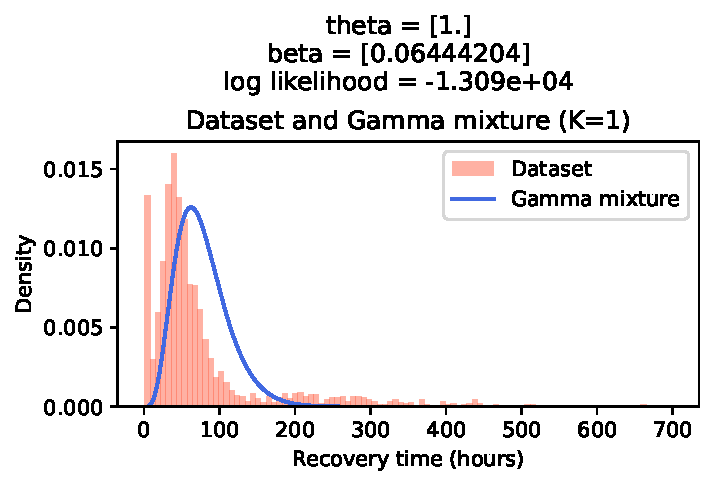
\includegraphics[width=0.8\linewidth]{hw5/img_output/p2_3_1mixtures.pdf}
    \end{figure}
    \begin{figure}[H]
        \centering
        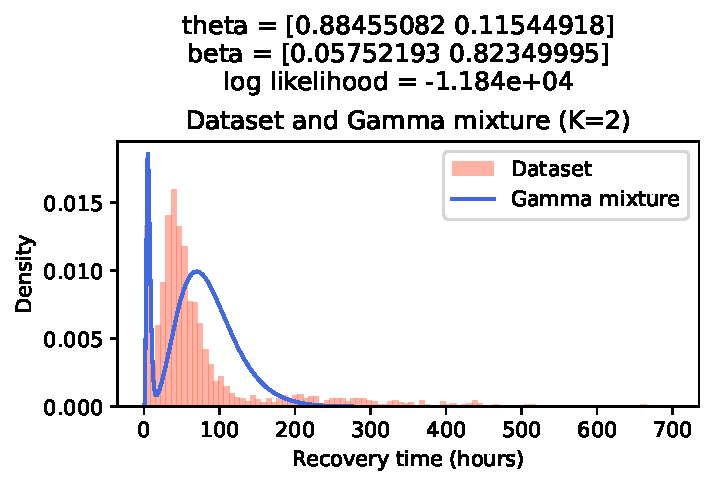
\includegraphics[width=0.8\linewidth]{hw5/img_output/p2_3_2mixtures.pdf}
    \end{figure}
    \begin{figure}[H]
        \centering
        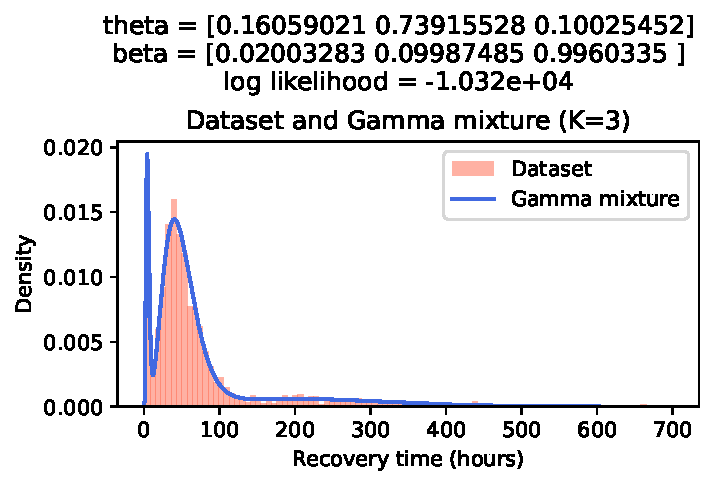
\includegraphics[width=0.8\linewidth]{hw5/img_output/p2_3_3mixtures.pdf}
    \end{figure}
    \begin{figure}[H]
        \centering
        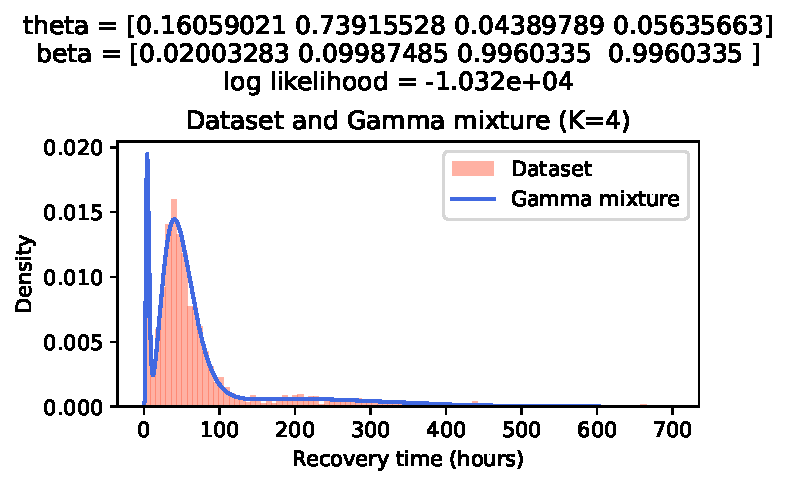
\includegraphics[width=0.8\linewidth]{hw5/img_output/p2_3_4mixtures.pdf}
    \end{figure}
    
    \item This matches what we see in the data. In the plot from part (1), we see a large proportion of the patients had recovery times around 2-3 days (48 - 72 hours), as indicated by the large peak in the distribution. However, we also see that there is a substantial peak around 0-10 hours, indicating that a large number of patients recovered quickly from the procedure. This corresponds with the doctors claim that some patients recover faster than normal. One possible explanation could be the quality of the surgery. If the procedure is extremely complex (but when done perfectly requires little recovery), it could be the case that a group of patients could have very short recovery times due to their surgery being performed perfectly while the average patient has a longer recovery time due to a complication in the difficult surgery. Another possible explanation could be that the recovery time of the surgery varies with patient health. The average person who does not exercise daily would probably take longer to recover physically than a young athlete who trains twice a day and maintains stellar health. If there was a number of athletes who underwent this procedure, then they could account for the group of patients who recovered faster.

    \item Yes. When we fit a three component mixture, a separate component appears that sits well beyond the normal 48 - 72 hour range and carries its own nontrivial weight.  If those slow recoveries were simply the extreme end of one distribution, adding components would not affect the fit or log likelihood of the model. Looking at our plots, we observe that the third gamma in the $K = 3$ mixture model isolates those long recoveries and has a higher likelihood and a better fit compared to $K = 2$. Therefore, there is evidence that these patients represent a different cluster.

    \item  Yes, the mixture modeling approach is appropriate for this task. Since the doctors want to distinguish between patients with typical and unusually long recovery times, then a mixture model is a natural choice since it would segment the population into latent subpopulations based on recovery behavior. Then, once these groups of similar patients have been identified, the doctors can explore what characteristics or indicators differentiate these groups.

    \item Using cluster membership alone to predict who will stay long in the hospital may be beneficial but also carries risks. On the plus side, a blood test that assigns patients to the long recovery cluster in advance could help flag those at risk and allocate resources accordingly. However, in practice, cluster labels derived from recovery time itself are not perfectly accurate and only probabilistic. Patients on the border between clusters (especially since the variance of the longer recovery cluster is large) may be misclassified and thus may not be given the proper care that they need. Thus, relying solely on that label can lead to more complications in patient care down the road. 
\end{enumerate}
\end{solution}

\newpage




\begin{problem}[PCA, 15 pts]

  For this problem you will implement PCA from scratch on the first 6000 images of the MNIST dataset. Your job is to apply PCA on MNIST and discuss what kind of structure is found. Implement your solution in \texttt{homework5.ipynb} and attach the final plots below. \\

  \noindent {\bfseries You will receive no points for code not included below or for using third-party PCA implementations (i.e. {\normalfont \texttt{scikit-learn}}).}
  \begin{enumerate}

    \item Compute the PCA. Plot the eigenvalues corresponding to the most
    significant 500 components in order from most significant to
    least. Make another plot that describes the cumulative proportion of
    variance explained by the first $k$ most significant components for
    values of $k$ from 1 through 500.  How much variance is explained by
    the first 500 components?  Describe how the cumulative proportion of
    variance explained changes with $k$.  Include this plot below.

    \item Plot the mean image of the dataset and plot an image
    corresponding to each of the first 10 principle components.  How do
    the principle component images compare to the cluster centers from
    K-means? Discuss any similarities and differences.  Include these
    two plots below.
    
    \textit{Reminder: Center the data before performing PCA.}

    \item Compute the reconstruction error on the dataset using the first 10 principal components. Then compute the reconstruction error when the reconstruction for each point is just the mean
    image of the dataset. How do these errors compare to
    the final objective loss achieved by using K-means on the dataset?
    Discuss any similarities and differences.

    For consistency in grading, define the error function as the squared L2
    norm of the difference between the true data and the reconstruction, averaged over all data points.
  
    \item Suppose you took the original matrix of principle components
    that you found $V$ and multiplied it on the right side by some rotation matrix $R$ (i.e., you considered the matrix $VR$).
    Would that change the quality of the reconstruction error in the
    last problem?  The interpretation of the components?  Why or why
    not?

    \item Let's recall the zipcode application in Homework 3.  A common
    application of PCA is to dimensionality reduction before running a
    classifier: You first project the data onto the first few PCA bases,
    and then you train a classifier from the projection to the output.
    \begin{enumerate}
      \item First, how might this be advantageous to just applying the classification algorithm directly, from both a robustness and efficiency perspective? 
      
      \item Second, recall from Homework 3 that adversaries can attack a classification algorithm by manipulating/perturbing the data; how could this approach help with such attacks?
    \end{enumerate}

    \item You are collaborating with a penmanship analysis expert.  They
    are able to identify the kind of pen used to make a mark by various
    characteristics such as the width of the line, its crispness, and
    the type (if any) of ink splatter.  They have heard that your
    machine learning helped automate reading zip codes for the post
    office; they are wondering if you can help automate the manual
    process of classifying pen types.
    \begin{enumerate}

      \item Does what the expert is describing correspond to some kind
      of hidden representation or latent variable?  Describe why or
      why not.
      
      \item Do you think PCA will help the expert?  Why or why not?
    \end{enumerate}
  \end{enumerate}
\end{problem}

\newpage

\begin{solution}
\begin{enumerate}
    \item The plots are below. The first 500 components explain around 95\% of the variance. However, we note that the first 150 components capture around 90\% of the variance. Thus, as we can see, the cumulative proportion of variance explained grows extremely quickly for small $k$ but grows exponentially slower as $k$ increases, following a diminishing return curve. 
    \begin{figure}[H]
        \centering
        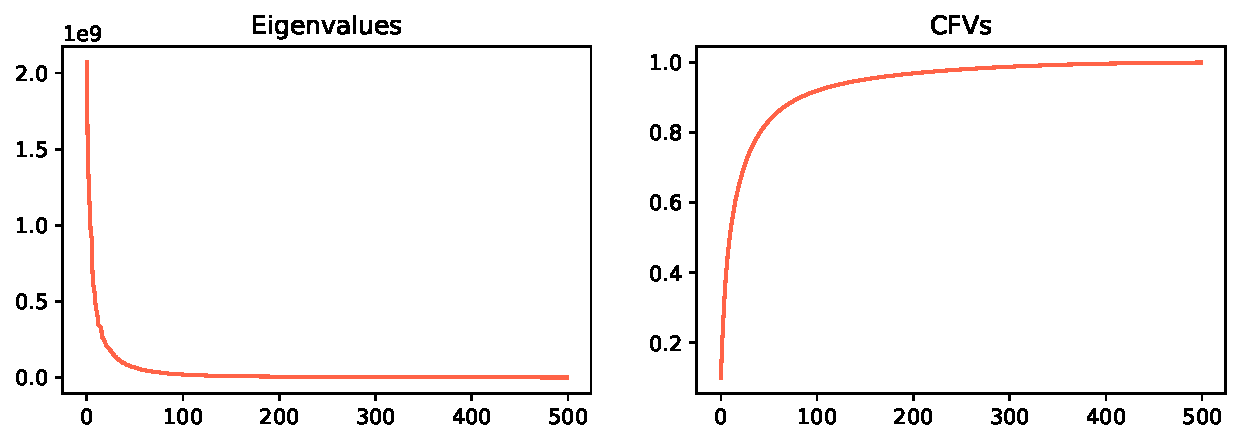
\includegraphics[width=0.9\linewidth]{hw5/img_output/p3_cfvs.pdf}
    \end{figure}
    
    \item Both the principle components and K-means images share the same structure of darker background and some white shape resembling a number in the center. However, the principle component images are much more blurry and washed out than the cluster centers from K-means. Moreover, the principle component images are more gray and do not resemble any singular digit, while the K-means images have more contrast and resemble a well formed digit. This is because the principle components together must capture the variance of all the digits in the dataset. Thus, it makes sense that their images are much less well formed and blurry since the components must capture a large proportion of the variance of all 10 digits present in the data. Meanwhile, the K-means clusters must individually represent a similar group of data points. Therefore, it makes sense that the K-means cluster centers will resemble digits much closer. 
    \begin{figure}[H]
        \centering
        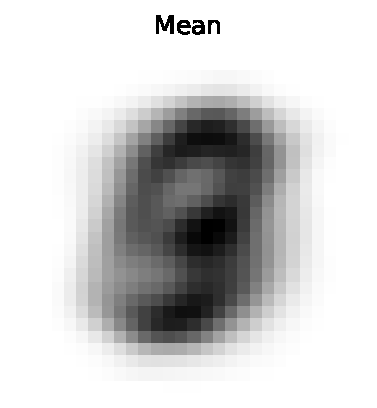
\includegraphics[width=0.3\linewidth]{hw5/img_output/p3_mean.pdf}
    \end{figure}
    \begin{figure}[H]
        \centering
        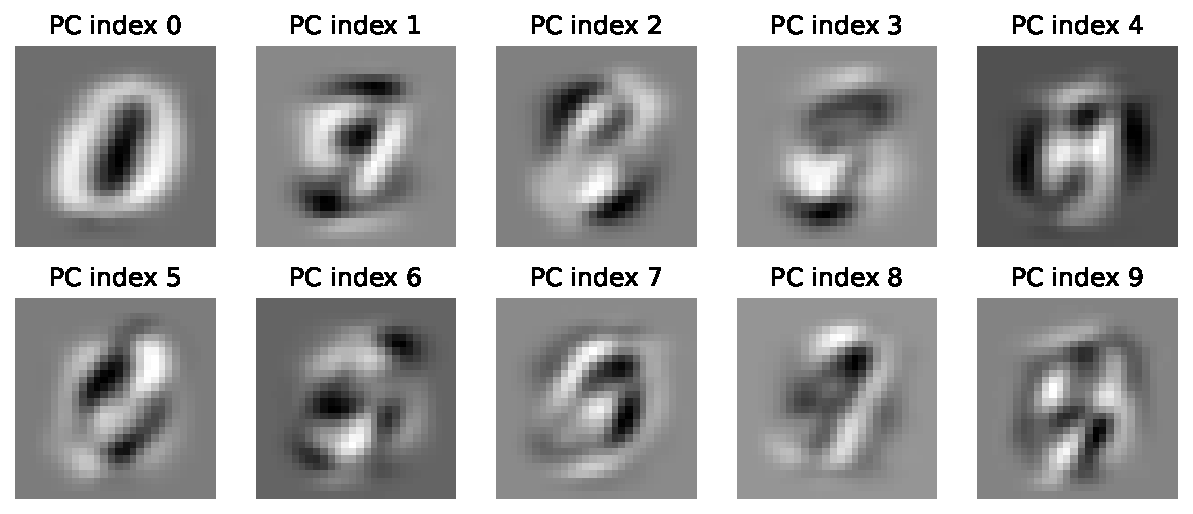
\includegraphics[width=0.9\linewidth]{hw5/img_output/p3_pcomps.pdf}
    \end{figure}
    
    \item The reconstruction error using the first 10 principal components is $1.731315e+06$. The reconstruction error using the mean image of the dataset is $3.436023e+06$. From TF Josh Park's Ed post, we know that the K-means Objective Loss is $2.6e+06$. Thus, the error using the first 10 principal components is lower than the K-means error while the error using just the mean image is higher than the K-means error. Intuitively this makes sense, since the CFV plot shows that the first ten principal components capture roughly 50\% of the total variance. Using just those ten components thus retains most of the important variation in each digit, resulting in lower errors. On the other hand, the K‑means algorithm represents each digit by its nearest centroid, which means it is vulnerable to individual variations among the data points (ie. how a digit is drawn compared to the centroid) which result in more error. Finally, the mean image has the highest error because it uses the single mean image for all ten digit classes, so it cannot capture any of the class specific or individual variations in how the digits are drawn.
    
    \item  If we replace $V$ with $VR$ for some rotation matrix $R$, the reconstruction error would remain exactly the same since the subspace spanned by the top $k$ columns (principal components) of $V$ is unchanged. However, this means that the individual columns of $VR$ will no longer be aligned with the directions of maximal variance. Thus, their interpretation as principal components is lost even though the reconstruction quality is identical.

    \item 
    \begin{enumerate}
        \item From an efficiency standpoint, projecting the data onto the top $k$ principal components reduces the input dimensionality, which leads to faster training and inference since the complexity and number of operations naturally scale with feature count (matrix multiplications involve larger matrices). In addition, in terms of robustness, PCA can help remove noise by discarding components that capture little variance -- these components probably correspond to irrelevant details or natural variance in data. By only keeping the largest components, we keep the overall trend in data while discarding much of the inherent noise in the data. Thus, PCA can help mitigate the risk of overfitting and thus help the classifier generalize better, especially when the original input space is very high dimensional.
    
        \item PCA can also help mitigate adversarial attacks by acting as a denoising or smoothing layer before classification. As mentioned in pset 3, adversaries can attack the algorithm by introducing subtle perturbations in the data, thus altering features in directions that a classifier is sensitive to. By projecting onto the top principal components, PCA discards those low variance directions that could include adversarial noise, therefore reducing the impact of the perturbation. This could force an adversary to introduce larger magnitude perturbations to "break through" the PCA which in turn could be easier to detect, thus potentially reducing the effectiveness of these adversarial attacks. While this is not a comprehensive defense, it introduces a kind of noise filter that can make classifiers less vulnerable to small adversarial distortions to the input.
    \end{enumerate}
    \item 
    \begin{enumerate}
        \item Yes. We cannot observe the kind of pen used directly from the image itself. However, we can observe characteristics like the line width, ink splatter, and crispness, which are all influenced by the kind of pen used to make the mark. Therefore, the pen type is a latent variable. 
    
        \item PCA could give the expert a quick, low dimensional summary of the dominant axes of variation in penmanship such as stroke width, ink splatter, or crispiness. That can be a useful first step for analysis since PCA will simplify a high dimensional dataset while preserving much of the variance of the data. In addition, PCA can reveal unexpected correlations useful to his process: if stroke width and pressure always vary together, then this relationship will appear in the principal components. However, the principal components will inevitably mix together multiple penmanship characteristics (ie. there won't be a component that corresponds to stroke width or type of ink splatter). Therefore, the expert won't be able to use PCA to automate the isolation of characteristics to automate their process. Moreover, small but significant details may be lost in the process of discarding low variance components. For example, if most ink splatter looks similar but tiny differences reveal the type of pen used, then this useful information could be lost in the PCA process.
\end{enumerate}

    
\end{enumerate}
\end{solution}

\begin{lstlisting}
import torch
import torchvision
import numpy as np
import matplotlib.pyplot as plt
%matplotlib inline
%config InlineBackend.figure_format = 'svg'

mnist_trainset = torchvision.datasets.MNIST(root='./data', train=True, download=True)  # download MNIST
N = 6000 

x = mnist_trainset.data[:N]  # select N datapoints
x = x.flatten(1)             # flatten the images
x = x.float()                # convert pixels from uint8 to float
x = x.numpy()              # uncomment to use numpy (optional)

def pca(x, n_comps=500):
    x_centered = x - np.mean(x, axis=0)
    U, S, Vt = np.linalg.svd(x_centered, full_matrices=False)
    pcomps = Vt[:n_comps, :]
    eigvals = (S**2)[:n_comps]

    return eigvals, pcomps

def calc_cfvs(eigvals):
    cfv = np.cumsum(eigvals) / np.sum(eigvals)
    return cfv

def calc_errs(x, pcomps):
    x_centered = x - np.mean(x, axis=0)

    x_recon_mean = np.zeros_like(x_centered)
    err_mean = np.mean(np.linalg.norm(x_centered - x_recon_mean, axis=1) ** 2)

    x_proj = np.dot(x_centered, pcomps.T)
    x_recon_pca = np.dot(x_proj, pcomps)
    err_pcomp = np.mean(np.linalg.norm(x_centered - x_recon_pca, axis=1) ** 2)

    return err_mean, err_pcomp

def plot_pic(pic, ax, title=''):
    x = pic.reshape(28, 28)
    ax.imshow(x, cmap='binary')
    ax.set_title(title)
    ax.axis('off')

def make_plots(eigvals, cfvs, x_mean, pcomps):
    # plot eigenvals and cfvs
    fig, (ax1, ax2) = plt.subplots(1, 2, figsize=(10, 3))
    ax1.plot(eigvals, color='tomato')
    ax1.set_title('Eigenvalues')
    ax2.plot(cfvs, color='tomato')
    ax2.set_title('CFVs')
    fig.savefig('img_output/p3_cfvs.pdf', bbox_inches = 'tight')

    # plot mean
    fig, ax = plt.subplots(1, 1, figsize=(3, 3))
    plot_pic(x_mean, ax, title='Mean')
    fig.savefig('img_output/p3_mean.pdf', bbox_inches = 'tight')

    # plot top 10 pcomps
    fig, axes = plt.subplots(2, 5, figsize=(10, 4))
    for i in range(10):
        plot_pic(pcomps[i], axes.flat[i], title=f'PC index {i}')
    fig.savefig('img_output/p3_pcomps.pdf', bbox_inches = 'tight')

# do PCA
eigvals, pcomps = pca(x)

# calculate CFVs
fcvs = calc_cfvs(eigvals)

first10 = pcomps[:10, :]

# print errors
err_mean, err_pcomp = calc_errs(x, first10)
print(f'Reconstruction error (using mean): {err_mean:3e}')  # 3.436022e+06
print(f'Reconstruction error (using mean and top 10 pcomps): {err_pcomp:3e}')  # 1.731315e+06

# make plots
make_plots(eigvals, fcvs, x.mean(0), pcomps)

\end{lstlisting}




\begin{problem}[Bayesian Networks, 10 pts]
  In this problem we explore the conditional independence
  properties of a Bayesian Network.  Consider the following Bayesian
  network representing a fictitious person's activities. Each random
  variable is binary (true/false).

  \begin{center}
    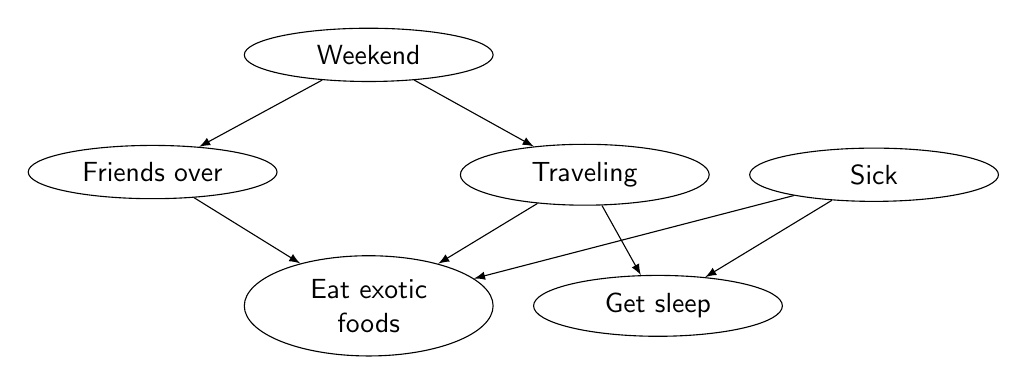
\begin{tikzpicture}[
      node distance=1cm and .5cm,
      bn/.style={draw,ellipse,text width=2cm,align=center}
        ]
      \node[bn] (w) {\attr{Weekend}};
      \node[bn,below right=of w] (t) {\attr{Traveling}};
      \node[bn,right=of t] (s) {\attr{Sick}};
      \node[bn,below left=of w] (f) {\attr{Friends over}};
      \node[bn,below right=of f] (eef) {\attr{Eat exotic foods}};
      \node[bn,right=of eef] (gs) {\attr{Get sleep}};
      \path (w) edge[-latex] (t)
      (w) edge[-latex] (f)
      (f) edge[-latex] (eef)
      (t) edge[-latex] (eef)
      (t) edge[-latex] (gs)
      (s) edge[-latex] (gs)
      (s) edge[-latex] (eef);
    \end{tikzpicture}
  \end{center}

  The random variables are:

  \begin{itemize}
  \item \attr{Weekend}: Is it the weekend?
  \item \attr{Friends over}: Does the person have friends over?
  \item \attr{Traveling}: Is the person traveling?
  \item \attr{Sick}: Is the person sick?
  \item \attr{Eat exotic foods}: Is the person eating exotic foods?
  \item \attr{Get Sleep}: Is the person getting sleep?
  \end{itemize}

  \medskip

  \noindent For the following questions, $A \perp B$ means that events A and B are independent and $A \perp B\mid C$ means that events A and B are independent conditioned on C. \\

  \noindent \textbf{Use the concept of d-separation} to answer the
  questions and show your work (i.e., state what the blocking path(s) is/are and what nodes block the path; or explain why each path is not blocked). For example, consider the following question and answer:
  \begin{itemize}
    \item[-] \textit{Example Question:} Is $\attr{Friends over} \perp \attr{Traveling}$? If NO, give intuition for why.
  
    \item[-] \textit{Example Answer:} NO. The path from Friends over -- Weekend -- Traveling is not blocked following the d-separation rules as we do not observe Weekend. Thus, the two are not independent. 
  \end{itemize}

  \noindent \textbf{Actual Questions:}

  \begin{enumerate}
    \item Is $\attr{Weekend} \perp \attr{Get Sleep}$?
      If NO, give intuition for why.

    \item Is $\attr{Sick} \perp \attr{Weekend}$?
      If NO, give intuition for why.

    \item Is $\attr{Sick} \perp \attr{Friends over}\given \attr{Eat exotic
      foods}$? If NO, give intuition for why.

    \item Is $\attr{Friends over} \perp \attr{Get Sleep}$? If NO, give
      intuition for why.

    \item Is $\attr{Friends over} \perp \attr{Get Sleep} \given
      \attr{Traveling}$? If NO, give intuition for why.

    \item Suppose the person stops traveling in ways that affect their
      sleep patterns.  Travel still
      affects whether they eat exotic foods.  Draw the modified network. (Feel free to reference the handout file for the commands for displaying the new network in \LaTeX).

    \item For this modified network, is $\attr{Friends over} \perp
      \attr{Get Sleep}$? If NO, give an intuition why.  If YES,
      describe what observations (if any) would cause them to no longer be
      independent.
  \end{enumerate}
\end{problem}

\begin{solution}
\begin{enumerate}
    \item No. We have the path from Weekend $\rightarrow$ Traveling $\rightarrow$ Get Sleep. However, since we do not condition on observing Traveling, then the path is not blocked following the d-separation rules. The intuition is that knowing it is the weekend makes it more probable that the person is traveling which then makes it more probable that they are getting sleep. Therefore, the two are not independent. 
    
    \item Yes. There are four paths from Sick to Weekend: Sick $\rightarrow$ Get Sleep $\leftarrow$ Traveling $\leftarrow$ Weekend, Sick $\rightarrow$ Get Sleep $\leftarrow$ Traveling $\rightarrow$ Eat Exotic foods $\leftarrow$ Friends over $\leftarrow$ Weekend, Sick $\rightarrow$ Eat exotic foods $\leftarrow$ Friends over $\leftarrow$ Weekend, and Sick $\rightarrow$ Eat exotic foods $\leftarrow$ Traveling $\leftarrow$ Weekend. 
    \\
    \\
    For the first path, Sick $\rightarrow$ Get Sleep $\leftarrow$ Traveling $\leftarrow$ Weekend, the subpath Sick $\rightarrow$ Get Sleep $\leftarrow$ Traveling is blocked at node Get Sleep since we do not observe Get Sleep. Therefore, the flow of information along this entire path is blocked.
    \\
    \\
    For the second path, Sick $\rightarrow$ Get Sleep $\leftarrow$ Traveling $\rightarrow$ Eat Exotic foods $\leftarrow$ Friends over $\leftarrow$ Weekend, the subpath Sick $\rightarrow$ Get Sleep $\leftarrow$ Traveling is blocked at node Get Sleep since we do not observe Get Sleep. Moreover, the subpath Traveling $\rightarrow$ Eat Exotic foods $\leftarrow$ Friends over is also blocked at Eat exotic foods since we do not observe Eat exotic foods. Therefore, the flow of information along this entire path is blocked.
    \\
    \\
    For the third path, Sick $\rightarrow$ Eat exotic foods $\leftarrow$ Friends over $\leftarrow$ Weekend, the subpath Sick $\rightarrow$ Eat exotic foods $\leftarrow$ Friends is blocked at the node Eat exotic foods since we do not observe Eat exotic foods. Therefore, the flow of information along this entire path is blocked.
    \\
    \\
    For the fourth path, Sick $\rightarrow$ Eat exotic foods $\leftarrow$ Traveling $\leftarrow$ Weekend, the subpath Sick $\rightarrow$ Eat exotic foods $\leftarrow$ Traveling is blocked at node Eat exotic foods since we do not observe Eat exotic foods. Therefore, the flow of information along this entire path is blocked.
    \\
    \\
    In every case, the flow of information is blocked along the path by the d-separation rules since we do not observe Eat exotic foods or Get sleep. Therefore, the two are independent.
    
    \item No. The path Sick $\rightarrow$ Eat exotic foods $\leftarrow$ Friends over is unblocked if we condition on observing Eat exotic foods. Intuitively, this is because if we observe Eat exotic foods, then observing that Sick is false increases the likelihood that Friends over is true because something must explain Eat exotic foods being true (either Traveling or Friends over). The same applies if we observe Friends over is false, which increases the likelihood that Sick is true. Therefore, the two are conditionally dependent.
    
    \item No. One path which is unblocked is Friends over $\leftarrow$ Weekend $\rightarrow$ Traveling $\rightarrow$ Get sleep. This is because the subpath Friends over $\leftarrow$ Weekend $\rightarrow$ Traveling is unblocked since we do not observe Weekend. In addition, the subpath Weekend $\rightarrow$ Traveling $\rightarrow$ Get sleep is unblocked since we do not observe Traveling. Intuitively, if the person has friends over, then it is more likely to be the weekend, which makes it more likely for the person is traveling, which finally makes it more likely that they will get sleep. Therefore, since there exists an unblocked path for information to flow from Friends over to Get sleep, then the two are not independent.
    
    \item Yes. The two paths from Friends over to Get sleep are Friends over $\leftarrow$ Weekend $\rightarrow$ Traveling $\rightarrow$ Get sleep and Friends over $\rightarrow$ Eat exotic foods $\leftarrow$ Traveling $\rightarrow$ Get sleep. 
    \\
    \\
    For the first path, Friends over $\leftarrow$ Weekend $\rightarrow$ Traveling $\rightarrow$ Get sleep, if we observe Traveling then the subpath Weekend $\rightarrow$ Traveling $\rightarrow$ Get sleep is blocked at the node Traveling according to the d-separation rules. Therefore, the flow of information along this first path from Friends over to Get sleep is blocked. 
    \\
    \\
    For the second path, Friends over $\rightarrow$ Eat exotic foods $\leftarrow$ Traveling $\rightarrow$ Get sleep, since Eat exotic foods is unobserved, then the flow of information along the subpath Friends over $\rightarrow$ Eat exotic foods $\leftarrow$ Traveling is blocked at the node Eat exotic foods by the d-separation rules. Therefore, the flow of information along the whole second path is blocked. 
    \\
    \\
    Thus, conditioned on observing traveling, the two are independent.
    \item 
    \noindent
    \begin{center}
    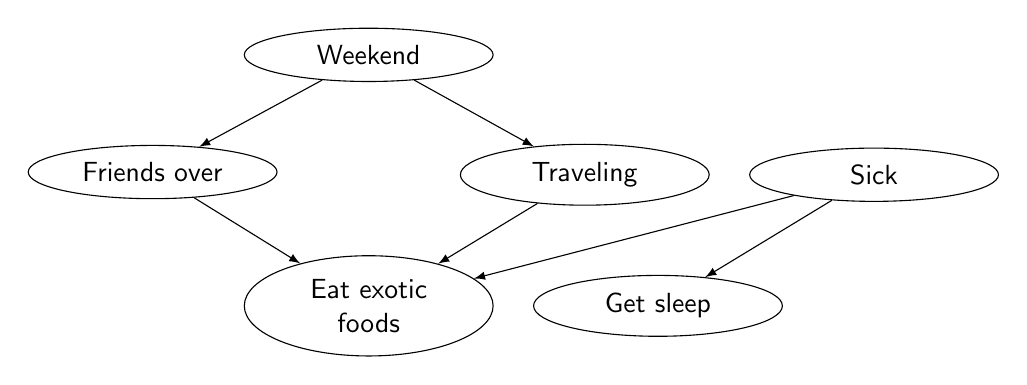
\begin{tikzpicture}[
      node distance=1cm and .5cm,
      bn/.style={draw,ellipse,text width=2cm,align=center}
        ]
      \node[bn] (w) {\attr{Weekend}};
      \node[bn,below right=of w] (t) {\attr{Traveling}};
      \node[bn,right=of t] (s) {\attr{Sick}};
      \node[bn,below left=of w] (f) {\attr{Friends over}};
      \node[bn,below right=of f] (eef) {\attr{Eat exotic foods}};
      \node[bn,right=of eef] (gs) {\attr{Get sleep}};
      \path (w) edge[-latex] (t)
      (w) edge[-latex] (f)
      (f) edge[-latex] (eef)
      (t) edge[-latex] (eef)
      (s) edge[-latex] (gs)
      (s) edge[-latex] (eef);
    \end{tikzpicture}
  \end{center}
  \item Yes. This is because there are two paths from Friends over to Get Sleep in this new network: Friends over $\leftarrow$ Weekend $\rightarrow$ Traveling $\rightarrow$ Eat exotic foods $\leftarrow$ Sick $\rightarrow$ Get sleep and Friends over $\rightarrow$ Eat exotic foods $\leftarrow$ Sick $\rightarrow$ Get sleep. 
  \\
  \\
  In the first path, we see that the subpath Traveling $\rightarrow$ Eat exotic foods $\leftarrow$ Sick is blocked at Eat exotic foods following the d-separation rules since we do not observe Eat exotic foods. Therefore, the flow of information along the entire first path is blocked. 
  \\
  \\
  For the second path, we see that the subpath Friends over $\rightarrow$ Eat exotic foods $\leftarrow$ Sick is blocked at node Eat exotic foods since both Friends over and Sick point into Eat exotic foods, and we do not observe Eat exotic foods. Therefore, the flow of information along the entire second path is blocked. 
  \\
  \\
  Thus, the two are independent.
\end{enumerate}
\end{solution}

\newpage
%%%%%%%%%%%%%%%%%%%%%%%%%%%%%%%%%%%%%%%%%%%%%
% Name and Calibration
%%%%%%%%%%%%%%%%%%%%%%%%%%%%%%%%%%%%%%%%%%%%%

\textbf{Name}: Jaray Liu

\textbf{Collaborators and Resources}: Ossimi Ziv

\end{document}